For an intruder the best path is not simply defined by the shortest path towards the target, but rather to avoid the guards an smarter path needs to be evaluated. SneakyThief algorithm is invented during the production of this research.
	%Workings of Sneakescape
			Sneakescape uses an evaluation function $s(x)$ which depends on the A-star's evaluation function $f(x)$ (see eq.~\ref{eq:astarevaluation}) and the summation heuristic functions toward the predators $h(G_i)$.In order to vary the importance of getting to the goal rather than escaping from the guards a weight value is assigned to the heuristic value of getting to the goal
			\begin{equation}
				\label{eq:sneakyscape}
			 	s(x,G) = c(x) + \alpha h(x) - \sum_{i=0}^n h(G_i)
			\end{equation} 
			Where $x$ is the coordinate of the target, $G$is the list of predators coordinates and $\alpha$ is the given weight to the tendency of moving towards the target. At every iteration the neighbour with the lowest $s(x,G)$ is chosen(see alg.~\ref{alg:sneakyscape}).
	\begin{algorithm}
	 \label{alg:sneakyscape}
				\KwData{Prey coordinate $t$; Set of predator coordinates $G$; Goal Coordinate $x$; evaluation function $s(x,G)$}
				\For{$n \in $ movable neighbours of $t$}{
				    Calculate $s(x,G)$\;
				}
				Return $\min_{s(x,G)}$ \;
				\caption{Sneakescape algorithm}
			\end{algorithm}
			
	\begin{figure}
	    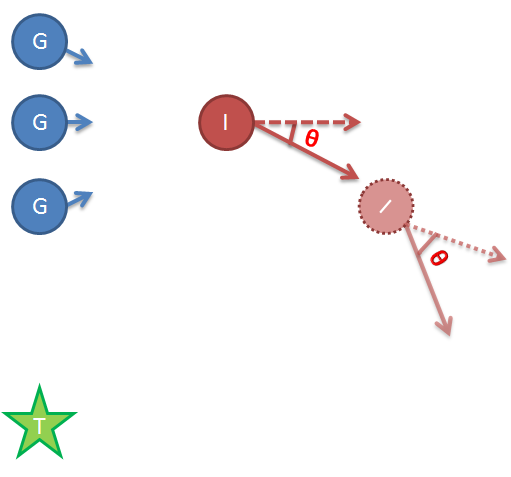
\includegraphics[width=\columnwidth]{SneakyStuff.PNG}
	    \caption{Sneakescape illustrative figure: where the intruder moves away from the guards and at the same time it has the tendency to go towards the target. $I$, $G$, and $T$ denote, intruder, guard, and target respectively. $\theta$ is the angle of move relative to the direction which leads to the furthest grid from all the guards.$\theta$ is directly proportional to the given weight $\alpha$, (see eq. \ref{eq:sneakyscape}).The dotted arrow indicates the move direction if the given weight to the target is $0$}
	\end{figure}
